\documentclass[12pt,aspectratio=43]{beamer}

%%%%%%%%%%%%%%%%%%%%%%%%%%%%%%%%%%%%%%%%%%%%%%%%%%
%   Paquetes de configuración basica del texto   %
%%%%%%%%%%%%%%%%%%%%%%%%%%%%%%%%%%%%%%%%%%%%%%%%%%
\usepackage[spanish,es-nodecimaldot]{babel}
\usepackage{babelbib}
\usepackage[T1]{fontenc}
\usepackage{listings}
\usepackage{multirow}
\usepackage{hyperref}
\usepackage{hyperxmp}
\usepackage{ifthen}

%%%%%%%%%%%%%%%%%%%%%%%%%%%%%%%%%%%%%%%%%%%%%%%%%%
%                   [listings]                   %
%   Configuración de vizualizacion del código    %
%%%%%%%%%%%%%%%%%%%%%%%%%%%%%%%%%%%%%%%%%%%%%%%%%%
\lstset{
	backgroundcolor=\color{lightgray!10},
	basicstyle=\ttfamily,
	extendedchars=true,
	showspaces=false,
	showstringspaces=false,
	captionpos=b,
	keywordstyle=\bfseries\color{cyan},
	commentstyle=\color{gray},
	stringstyle=\color{orange},
	escapeinside={!>}{<!},
	language=[LaTeX]TeX }

%%%%%%%%%%%%%%%%%%%%%%%%%%%%%%%%%%%%%%%%%%%%%%%%%%
%     Paquetes de configuración graficos del     %
%                   documento                    %
%%%%%%%%%%%%%%%%%%%%%%%%%%%%%%%%%%%%%%%%%%%%%%%%%%
\usepackage{graphicx}
\usepackage{tikz}
\usetikzlibrary{babel,shadows}
\usepackage{xcolor}
\usepackage{pdfpages}
\usepackage{animate}

\usepackage{ifxetex}
\ifxetex
	\usepackage[no-math]{fontspec}
	\setmainfont{AncizarSans}[
		Path = ../Fuentes/,
		Extension = .otf,
		BoldFont = *-B,
		ItalicFont = *-I,
		BoldItalicFont = *-BI ]
	\setmonofont{UbuntuMono}[
		Path = ../Fuentes/,
		Extension = .ttf,
		BoldFont = *-B,
		ItalicFont = *-I,
		BoldItalicFont = *-BI ]
	\newcommand{\lmr}{\fontfamily{lmr}\selectfont}
	\newcommand{\lmss}{\fontfamily{lmss}\selectfont}
	\newcommand{\lmtt}{\fontfamily{lmtt}\selectfont}
\fi

%%%%%%%%%%%%%%%%%%%%%%%%%%%%%%%%%%%%%%%%%%%%%%%%%%
%           Configuraciones de Beamer            %
%%%%%%%%%%%%%%%%%%%%%%%%%%%%%%%%%%%%%%%%%%%%%%%%%%
\definecolor{Igreen}{RGB}{148,180,59}
\definecolor{Ired}{RGB}{166,24,49}

\setbeamertemplate{navigation symbols}{}

\setbeamertemplate{itemize items}{\color{Igreen}\raisebox{.45ex}{\rule{.6ex}{.6ex}}}

\usefonttheme{professionalfonts}
\usefonttheme{serif}
\setbeamercolor{frametitle}{fg=Ired,bg=Igreen!50}
\setbeamercolor{alerted text}{fg=Ired}
\setbeamertemplate{enumerate item}{\color{Igreen}\bfseries\arabic{enumi}.}
\setbeamertemplate{enumerate subitem}{\color{Igreen}\bfseries\arabic{enumi}.\arabic{enumii}.}

\makeatletter
\newcommand{\ifratio}[2]{
	\ifthenelse
	{\lengthtest{\beamer@paperwidth=16cm} \AND \lengthtest{\beamer@paperheight=9cm}}
	{#1}
	{#2} }
\makeatother

\setbeamertemplate{title page}{
	\begin{tikzpicture}[overlay,remember picture]
	\path (current page.north west) ++(0.5cm,-0.5cm) node[below right] {
\includegraphics[height=1.25cm]{../Escudo_UN}};
	\path (current page.north east) ++(-0.5cm,-0.5cm) node[below left] {\parbox[c][1.25cm][c]{\widthof{\Large \insertsubtitle}}{\Large \insertsubtitle}};
	\end{tikzpicture}
	
	\vfill
	\begin{center}
		{\Huge\inserttitle}\\
		\bigskip
		\insertauthor
	\end{center}
	\vfill
}

%%%%%%%%%%%%%%%%%%%%%%%%%%%%%%%%%%%%%%%%%%%%%%%%%%
%         Información de la presentación         %
%%%%%%%%%%%%%%%%%%%%%%%%%%%%%%%%%%%%%%%%%%%%%%%%%%

\title{Editores y Compiladores}
\subtitle{Curso Libre de {\lmr\LaTeX}}
\author{Joar Esteban Buitrago Carrillo}
\institute{Universidad Nacional de Colombia}
\date{}
\logo{
\includegraphics[height=0.75cm]{../Escudo_UN}}
\hypersetup{
	pdfcopyright={Esta obra está bajo una licencia de Creative Commons Reconocimiento-CompartirIgual 4.0 Internacional.},
	pdflicenseurl={https://creativecommons.org/licenses/by-sa/4.0/deed.es}
}

\begin{document}
\begin{frame}[plain]
\titlepage
\end{frame}

{
\setbeamercolor{background canvas}{bg=}
\begin{frame}
\ifratio
	{\includepdf[pages=2]{../Licencia_Diapositiva.pdf}}
	{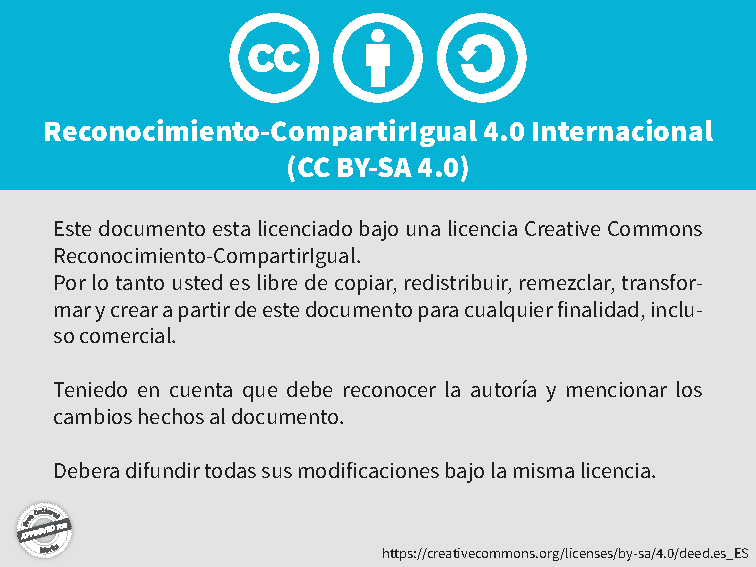
\includepdf[pages=1]{../Licencia_Diapositiva.pdf}}
\end{frame}
}

\section{Editores}
\begin{frame}{Editores}{}
La comunidad de {\lmr\LaTeX} ha diseñado una gran variedad de editores para hacer las tareas de edición de cualquier documento mucho más sencillas, y fáciles.\pause\\[2em]

Cada uno de ellos posee una gran variedad de características. Puedes ir analizando cada uno, y elegir el que más se acomode a tus gustos y necesidades.
\end{frame}

\newcommand{\TeXmaker}{{\lmr\TeX} \textit{\lmss MAKER}}
\subsection{TeXmaker}
\begin{frame}{\TeXmaker}{}
\begin{center}
	
\includegraphics[height=2cm]{TeXmaker_Logo}\hspace{0.125cm}\parbox[b][2cm][c]{\widthof{\huge\TeXmaker}}{\huge\TeXmaker}
\end{center}

Página web: http://www.xm1math.net/texmaker/
\end{frame}

\begin{frame}{\TeXmaker}{}
{\TeXmaker} es un editor gratuito licenciado bajo GPL.\pause\\[1em]

Incluye:
\begin{itemize}[<+->]
	\item Soporte a Unicode.
	\item Corrección Ortográfica.
	\item Auto-completado.
	\item Plegado de código.
	\item Un visor integrado con soporte de sincronización.
\end{itemize}
\end{frame}

\begin{frame}[plain]{}{}
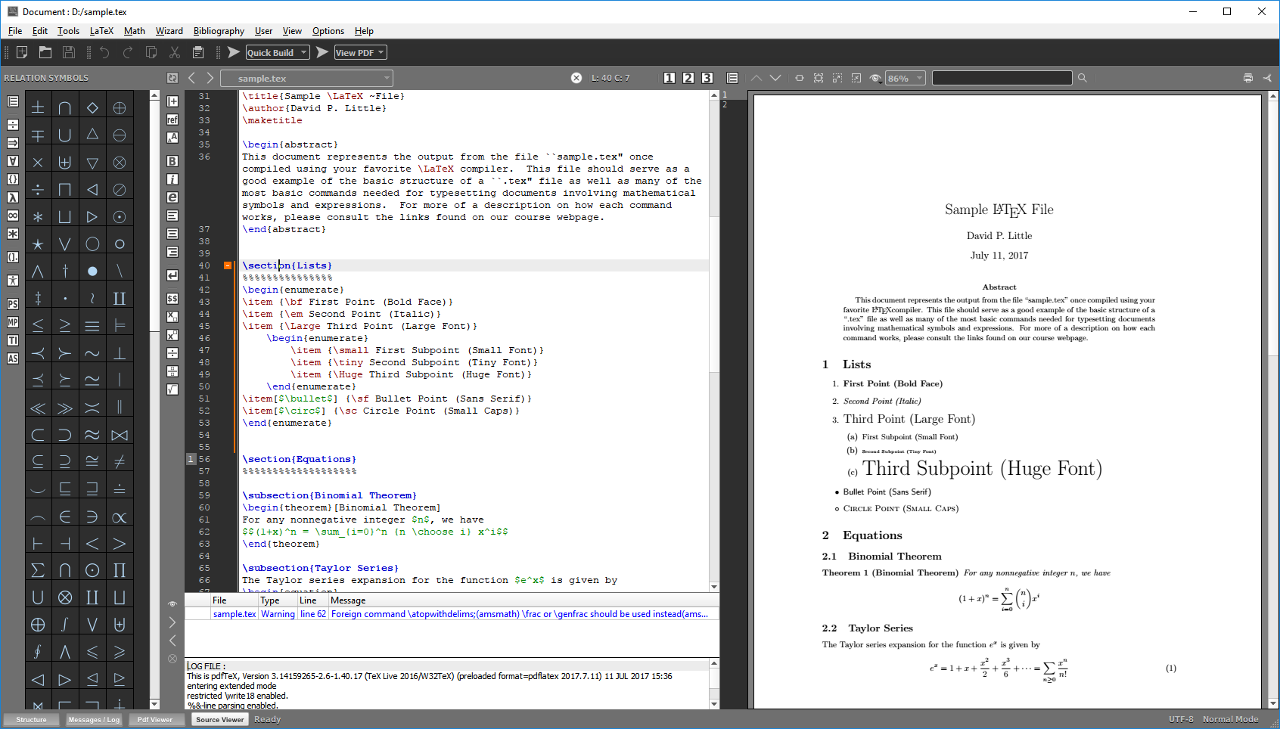
\includegraphics[width=\linewidth]{TeXmaker_Screen}
\end{frame}

\newcommand{\TeXstudio}{\lmr\TeX\fontshape{ui}\selectfont\lmr studio}
\subsection{TeXstudio}
\begin{frame}{\TeXstudio}{}
\begin{center}
	
\includegraphics[height=2cm]{TeXstudio_Logo}\hspace{0.125cm}\parbox[b][2cm][c]{\widthof{\huge\TeXstudio}}{\huge\TeXstudio}
\end{center}

Página web: https://www.texstudio.org/
\end{frame}

\begin{frame}[fragile]{\TeXstudio}{}
{\TeXstudio} es un editor gratuito licenciado bajo GPL.\\
Es derivado de {\TeXmaker}.\pause\\[1em]

Incluye:
\begin{itemize}[<+->]
	\item Soporte Unicode.
	\item Soporte a directivas \lstinline| % !TeX|
	\item Corrección Ortográfica.
	\item Auto-completado.
	\item Plegado de código.
	\item Un visor integrado con soporte de sincronización.
\end{itemize}
\end{frame}

\begin{frame}[plain]{}{}
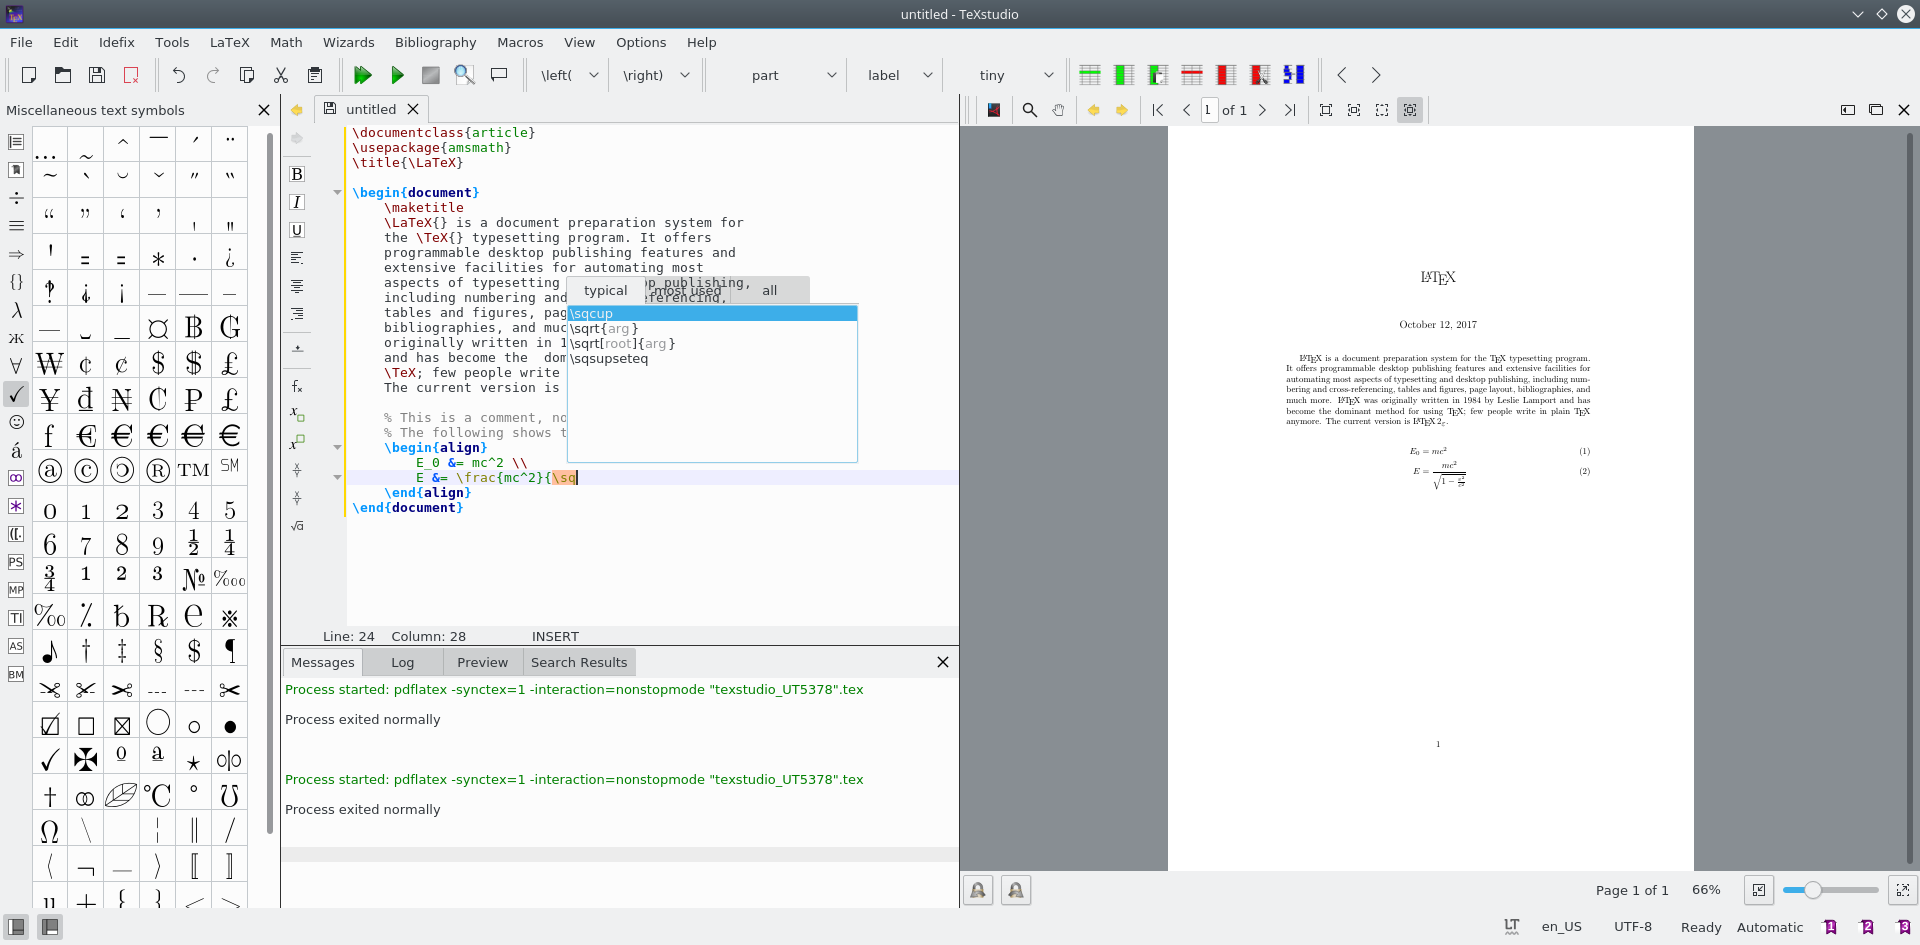
\includegraphics[width=\linewidth]{TeXstudio_Screen}
\end{frame}

\newcommand{\LyX}{\lmr L\hspace{-0.3ex}\raisebox{-0.5ex}{Y}\hspace{-0.3ex}X}
\subsection{LyX}
\begin{frame}{\LyX}{}
\begin{center}
	
\includegraphics[height=2cm]{LyX_Logo}\hspace{0.125cm}\parbox[b][2cm][c]{\widthof{\huge\LyX}}{\huge\LyX}
\end{center}

Página web: https://www.lyx.org/
\end{frame}

\newcommand{\AUCTeX}{\lmr AUC{\TeX}}
\subsection{AUCTeX}
\begin{frame}{\AUCTeX}{}
\begin{center}
	
\includegraphics[height=2cm]{AUCTeX_Logo}\hspace{0.125cm}\parbox[b][2cm][c]{\widthof{\huge\AUCTeX}}{\huge\AUCTeX}
\end{center}

Página web: https://www.gnu.org/software/auctex/
\end{frame}

\newcommand{\Kile}{\lmr Kile}
\subsection{Kile}
\begin{frame}{\Kile}{}
\begin{center}
	
\includegraphics[height=2cm]{Kile_Logo}\hspace{0.125cm}\parbox[b][2cm][c]{\widthof{\huge\Kile}}{\huge\Kile}
\end{center}

Página web: https://kile.sourceforge.io/
\end{frame}

\newcommand{\TeXmacs}{\lmr\TeX macs}
\subsection{TeXmacs}
\begin{frame}{\TeXmacs}{}
\begin{center}
	
\includegraphics[height=2cm]{TeXmacs_Logo}\hspace{0.125cm}\parbox[b][2cm][c]{\widthof{\huge\TeXmacs}}{\huge\TeXmacs}
\end{center}

Página web: https://kile.sourceforge.io/
\end{frame}

\section{Compiladores}
\begin{frame}{Compiladores}{}
Al trabajar con {\lmr\LaTeX} es necesario escoger un compilador que se acomode a tus gustos y tus necesidades.\pause\\[2em]

Estudiaremos solamente 4 compiladores.
\end{frame}

\subsection{\LaTeX}
\begin{frame}{\lmr\LaTeX}{}
\begin{center}
	\Huge\lmr\LaTeX
\end{center}
\end{frame}

\subsection{PDF\LaTeX}
\begin{frame}{\lmr PDF\LaTeX}{}
\begin{center}
	\Huge\lmr PDF\LaTeX
\end{center}
\end{frame}

\newcommand{\XeTeX}{\lmr X\hspace{-0.3ex}\raisebox{-0.5ex}{\reflectbox{E}}\hspace{-0.4ex}{\TeX}}
\newcommand{\XeLaTeX}{\lmr X\hspace{-0.3ex}\raisebox{-0.5ex}{\reflectbox{E}}\hspace{-0.25ex}{\LaTeX}}
\subsection{XeLaTeX}
\begin{frame}{{\XeTeX} y {\XeLaTeX}}{}
\begin{center}
	\Huge{\XeTeX} y {\XeLaTeX}
\end{center}
\end{frame}

\newcommand{\LuaTeX}{\lmr Lua\hspace{-0.4ex}{\TeX}}
\newcommand{\LuaLaTeX}{\lmr Lua\hspace{-0.1ex}{\LaTeX}\relax}
\subsection{LuaLaTeX}
\begin{frame}{{\LuaTeX} y {\LuaLaTeX}}{}
\begin{center}
	\includegraphics[height=2cm]{LuaTeX_Logo}\hspace{0.125cm}\parbox[b][2cm][c]{\widthof{\Huge{\LuaTeX} y {\LuaLaTeX}}}{\Huge{\LuaTeX} y {\LuaLaTeX}}
\end{center}
\end{frame}
\end{document}